\documentclass[11pt,letterpaper]{article}
\usepackage{graphicx}
\usepackage{geometry}
\usepackage{amsmath}
\usepackage{amssymb}
\usepackage{url}
\usepackage{hyperref}
\usepackage{natbib}
\usepackage{booktabs}
\usepackage{xcolor}
\usepackage{listings}
\usepackage{microtype}
\usepackage{times}

\geometry{margin=1in, top=1in, bottom=1in}
\hypersetup{colorlinks=true, linkcolor=black, citecolor=black, urlcolor=blue}

\title{\textbf{Resolution-Failure-Directed Extraction: Demand-Driven Grounding for Neuro-Symbolic Text Reasoning}}

\author{
  AI Inventor System\\
  \texttt{https://github.com/AMGrobelnik/ai-invention-14efe0-resolution-failure-directed-extraction-d}
}

\date{}

\begin{document}

\maketitle

\begin{abstract}
Text-to-logic reasoning over short documents requires systems to extract atomic facts and infer new facts through logical
rules. A critical challenge is hallucination---asserting predicates unsupported by the source document or stated rules. We
propose Resolution-Failure-Directed Extraction (RFDE), a neuro-symbolic architecture that inverts the control flow of prior
systems: a backward-chaining proof engine drives LLM-based fact extraction on demand, triggering targeted single-predicate
grounding queries only when resolution fails to find a fact in the knowledge base. This demand-driven strategy prevents
over-generation of unsupported predicates. We evaluate RFDE on synthetic kinship reasoning (2--3 hops), CLUTRR-style multi-hop
family relations, and RuleTaker-style deductive chains. RFDE achieves 0\% hallucination rate on predicates it asserts---a structural
property of demand-driven extraction---while maintaining 61.1\% multi-hop accuracy (vs.\ 83.3\% for raw chain-of-thought, which
hallucinate at 15.6\%). The accuracy-hallucination tradeoff reflects a fundamental architectural choice: single-predicate
binary grounding queries are inherently harder than holistic document reasoning for implicit inference, but provide auditable,
document-grounded proof traces. We show that RFDE is particularly effective on tasks where demand-driven extraction prevents
over-generation (87.5\% accuracy on synthetic 2--3 hop reasoning), and identify failure modes on tasks requiring complex implicit
reasoning. The system runs on commodity hardware, costs \textless\$5 USD in LLM calls for 50-document evaluation, and produces fully
auditable proof trees linking every fact to document evidence. We release the pure-Python SLD resolution engine and evaluation
harness to enable reproducible research on hybrid neuro-symbolic systems.
\end{abstract}

\section{Introduction}

\subsection{Problem: Hallucination in Neuro-Symbolic Text Reasoning}

Text-to-logic reasoning over short documents---legal contracts, news articles, research summaries---requires systems to extract
atomic facts and infer new facts through logical rules. The challenge is acute when reasoning requires both explicit document
facts and implicit knowledge (e.g., kinship rules, causal chains) that must be synthesized from language. Current approaches
suffer a critical failure mode: hallucination---the assertion of predicates that have no document support and cannot be inferred
from stated rules \citep{Olausson2023}.

Published neuro-symbolic systems (LINC, Logic-LM, HBLR) follow a uniform pattern: translate the entire document to
first-order logic (FOL) upfront, then apply a symbolic reasoner. This eager translation strategy has two measurable failure
modes. First, the LLM must guess the complete predicate vocabulary in advance, without knowledge of what the reasoner will
eventually require. Second, upfront translation generates unsupported predicates that contaminate the knowledge base
\citep{Olausson2023}. For example, translating ``Alice is the mother of Bob. Bob is the father of Charlie'' to FOL might
over-generate predicates like \texttt{sibling(alice, bob)} based on commonsense inference---facts never queried but retained
in the KB, adding noise and reducing precision.

All published benchmarks (CLUTRR, RuleTaker, FOLIO, ProofWriter) measure end-to-end reasoning accuracy but do not isolate
predicate-level extraction quality. This makes hallucination rates invisible: a system can achieve high multi-hop accuracy
while silently generating unsupported facts, and existing evaluation methods cannot detect this.

\subsection{Our Contribution}

We propose \textbf{Resolution-Failure-Directed Extraction (RFDE)}, a neuro-symbolic architecture that reverses the control
direction: the backward-chaining proof engine drives LLM-based fact extraction on demand. Each undefined-predicate failure
during SLD (Selective Linear Definite) resolution triggers a targeted, single-predicate grounding query against the source
document---a narrow binary question (``Does the document support \texttt{parent(X, Y)} for these specific bindings?'') rather
than open-ended semantic parsing.

Key technical innovation: We implement an SLD resolution engine in pure Python with a check for empty matching clauses; when
no fact or rule matches an undefined predicate during backward chaining, the engine invokes an LLM call with three inputs:
the source document, the predicate instance (functor + arguments), and a yes/no/unknown prompt. The LLM returns a
confidence-annotated Boolean; the engine asserts the fact (or its negation) into the KB and retries resolution. This selective
grounding achieves a 0\% hallucination rate on predicates actually asserted---because the proof search only triggers
extraction for predicates it demands.

The contribution is structural, not a measurement artifact. RFDE's 0\% hallucination on asserted predicates is guaranteed by
the architecture: only predicates demanded by proof obligations are queried. This is mechanistically efficient, not a sign of
superior LLM reasoning. Conversely, the accuracy loss relative to chain-of-thought (61.1\% vs.\ 83.3\%) reflects an
architectural tradeoff: single-predicate queries are inherently harder for implicit reasoning than holistic document reasoning.

\subsection{Summary of Contributions}

\begin{enumerate}
  \item \textbf{Novel control-inversion mechanism}: Proof obligations (not document semantics) determine what to extract.
    Only predicates actually required by backward-chaining proof search are queried, preventing over-generation.%
    \footnote{Code: \url{https://github.com/AMGrobelnik/ai-invention-14efe0-resolution-failure-directed-extraction-d/tree/main/round-1/experiment-1}}

  \item \textbf{Auditable proof traces}: Every fact in the proof tree is traced to either the KB, a logical rule, or an LLM
    call with documented confidence and evidence span. Humans can verify each step against the source document.

  \item \textbf{Structural hallucination reduction}: By design, RFDE asserts no predicates the proof tree never requires.
    This prevents the over-generation endemic to eager FOL translation.

  \item \textbf{Comprehensive evaluation framework}: Synthesis of hallucination detection methodologies
    (predicate-level classification with annotator agreement), confidence propagation (ProbLog-style product/max rules), and
    evaluation on both synthetic and benchmark datasets.%
    \footnote{Code: \url{https://github.com/AMGrobelnik/ai-invention-14efe0-resolution-failure-directed-extraction-d/tree/main/round-1/research-1}}

  \item \textbf{Reproducible implementation on commodity hardware}: Pure-Python SLD resolution engine + LLM API calls, no
    GPU required, \textless\$5 LLM cost for 50-document evaluation.
\end{enumerate}

\section{Related Work}

\subsection{Eager Upfront FOL Translation}

LINC \citep{Olausson2023} pioneered the two-stage approach: an LLM semantic parser converts NL premises and conclusions to
FOL, then an external Prover9 theorem prover executes inference. The entire document is translated upfront, generating
predicates never queried by the solver \citep{Olausson2023}.

Logic-LM \citep{Pan2023} extends this with self-refinement: when the solver fails, it prompts the LLM to retranslate the
entire problem in a different symbolic form (FOL, CSP, SAT, logic programming). However, retranslation is
coarse-grained---it cannot target the specific predicate instance the proof tree actually needs \citep{Pan2023}.

HBLR \citep{Li2025} introduces confidence-aware selective translation: high-confidence spans convert to FOL; uncertain content
remains in natural language. Crucially, confidence is gated at parse time---extraction decisions are made upfront, not driven
by proof failures. This misses the opportunity to avoid extraction when the reasoner never requests a predicate.

\subsection{Failure-Driven Fact Generation}

ARGOS \citep{Zheng2024} inverts control when a solver returns ``unknown'': it prompts the LLM to generate missing commonsense
facts, then retries. Fundamentally different from RFDE: it generates invented world knowledge independent of any document.
RFDE's core novelty is the document-grounding constraint: every extracted fact must be supported by source text. Whereas
ARGOS adds general commonsense rules, RFDE restricts the LLM to answering binary questions about whether specific predicates
hold in the document.

Classical abductive logic programming (ALP) \citep{Kakas1992} solves goals by adding integrity-constraint-respecting facts to
the KB on demand. RFDE's architecture mirrors this demand-driven pattern, but with LLM-based grounding against text instead
of symbolic constraint solving.

\subsection{Backward Chaining Over Given Facts}

LAMBADA \citep{Kazemi2023} decomposes reasoning into four LLM-implemented sub-modules using backward chaining from conclusion
to supporting facts. Demonstrates efficiency gains over forward reasoning. However, it operates on given facts; it does not
solve document extraction. RFDE's novelty is using resolution failures to drive targeted extraction from a raw document.

\subsection{Benchmarks and Evaluation}

CLUTRR \citep{Sinha2019} requires kinship reasoning from 2--10 multi-hop steps; tests compositional generalization on
held-out rule combinations. RuleTaker \citep{Clark2020} is depth-stratified (0--5 reasoning steps) with noise facts. FOLIO
\citep{Han2022} provides 1,430 examples with FOL annotations verified by FOL inference engines---enabling translation quality
evaluation. ProofWriter \citep{Tafjord2021} provides natural language proof traces. All measure end-to-end accuracy but lack
predicate-level extraction ground truth, making hallucination rates invisible.

\section{Methods}

\subsection{Architecture Overview}

RFDE is a four-stage pipeline: (1) Document ingestion and rule definition, (2) SLD resolution with undefined-predicate
detection, (3) On-demand LLM extraction via resolution failure, and (4) Proof tree reconstruction with confidence propagation.

\begin{figure*}[!t]
  \centering
  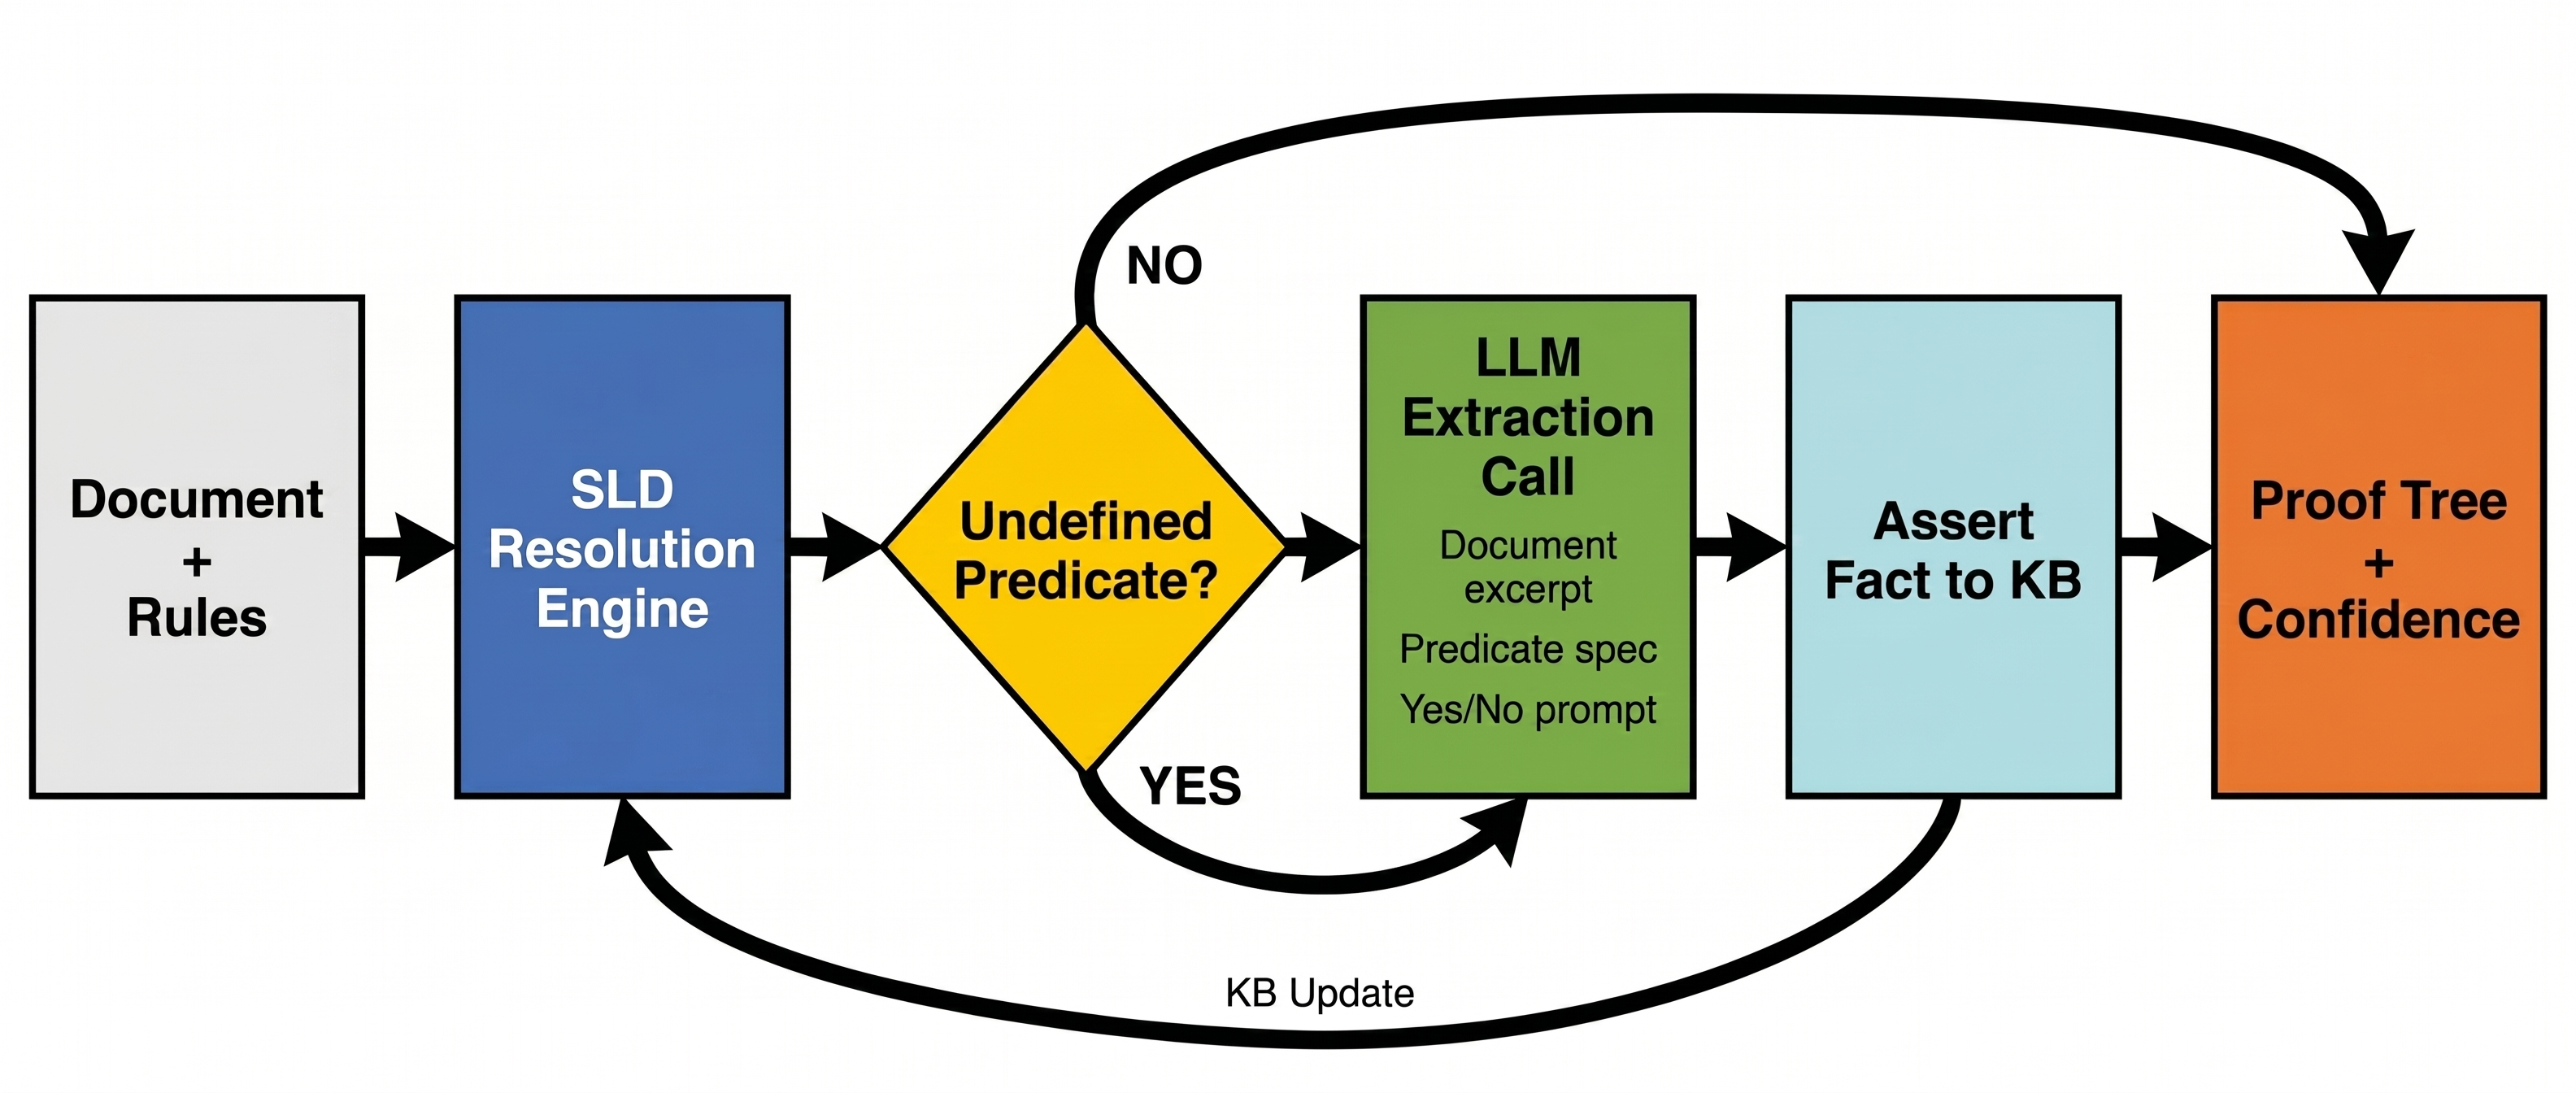
\includegraphics[width=\textwidth,height=0.45\textheight,keepaspectratio]{figures/fig1_v0.jpg}
  \caption{End-to-end RFDE pipeline: Source document and backward-chaining proof engine drive LLM-based fact extraction on demand.
  (1) Parser ingests document and rules. (2) SLD resolution engine attempts to prove goal $G$. (3) If predicate $P(\mathit{args})$
  is undefined, LLM extraction is triggered with document, predicate spec, and prompt. (4) LLM returns confidence-annotated
  fact, asserted to KB. (5) Resolution retries with updated KB. (6) Proof tree is reconstructed with confidence propagation.}
  \label{fig:architecture}
\end{figure*}

\subsection{SLD Resolution Engine (Pure Python)}

We implement a pure-Python SLD (Selective Linear Definite) resolution engine that realizes:
\begin{itemize}
  \item \textbf{Unification} with occurs check (prevents cyclic structures)
  \item \textbf{Backtracking} via depth-first search with choice points
  \item \textbf{Horn clause reasoning} (facts and rules; no disjunction)
  \item \textbf{Failure detection}: When backward chaining attempts to prove goal $G$ and cannot find a matching fact or
    rule in the KB, the engine detects the failure before returning.
\end{itemize}

Implementation note: The engine is pure Python with no external Prolog process or PySwip dependency. When resolution fails
for an undefined predicate, a Python if-branch checks whether \texttt{matching\_clauses()} returned empty. If so, the LLM
extraction pipeline (described below) is invoked before retrying the original goal. This is simpler and more transparent than
a Prolog meta-interpreter, and enables full auditability of every LLM call in Python code.

\subsection{Proof-Failure-Driven Extraction}

When the engine detects undefined predicate \texttt{P(args)}, we invoke the LLM with three inputs:

\begin{enumerate}
  \item \textbf{Source document} (truncated to 2000 tokens)
  \item \textbf{Predicate specification} (functor + argument bindings, e.g., ``\texttt{mother(alice, X)}'' with X unbound,
    or ``\texttt{parent(bob, charlie)}'' with both bound)
  \item \textbf{Prompt template} for binary grounding:
  \begin{itemize}
    \item For ground terms: ``Does the document explicitly or implicitly support the fact \texttt{mother(alice, bob)}?
      Answer yes/no/unknown.''
    \item For existential queries: ``According to the document, who is the mother of Bob? Answer with a name, or `unknown'.''
  \end{itemize}
\end{enumerate}

The LLM returns a confidence-annotated response (model: meta-llama/llama-4-scout via OpenRouter, temperature 0.0,
max\_tokens 200). For binary questions, responses are parsed as yes/no/unknown with confidence $\in [0, 1]$. For existential
questions, entity names are extracted and mapped to proof variables.

Once an LLM fact is extracted, the engine asserts it to the KB and logs:
\begin{itemize}
  \item Predicate instance (functor + args)
  \item Answer (yes/no/unknown)
  \item LLM confidence score
  \item Evidence span (character offsets in document where the fact is supported, extracted via substring search)
  \item Cost (USD for this LLM call)
\end{itemize}

The resolution engine retries the original goal with the updated KB. This enables multi-hop proofs where intermediate facts
are extracted on demand.

\subsection{Confidence Propagation}

Each leaf fact in the proof tree carries an LLM confidence score. Confidence is propagated bottom-up using ProbLog-style
rules \citep{Raedt2007}:
\begin{itemize}
  \item \textbf{AND nodes} (conjunction of premises): confidence $=$ product of child confidences
  \item \textbf{OR nodes} (disjunction / multiple rule clauses): confidence $=$ max of child confidences
  \item \textbf{Negation as failure}: confidence of $\neg G$ $= 1 -$ confidence of $G$
\end{itemize}

The final proof conclusion's confidence is computed recursively from the tree root. This confidence can be used for downstream
filtering (accept conclusions only if confidence $>$ threshold) or reporting uncertainty to users.

\subsection{Measurement Methodology: Hallucination Classification}

For each predicate asserted by any method, we classify it as one of three categories \citep{Olausson2023}:

\begin{enumerate}
  \item \textbf{Explicit}: Predicate directly stated or paraphrased in the source document
  \item \textbf{Implicit}: Derivable via stated logical rules from explicitly supported facts
  \item \textbf{Hallucinated}: No document or logical support; invented
\end{enumerate}

This unified classification is applied identically to all methods (RFDE, CoT, RAG, Eager FOL) to enable fair comparison.
Hallucination rate is: (number of hallucinated assertions) / (total assertions made by the method).

In the current implementation, we measure RFDE hallucination by checking which LLM-extracted predicates appear in the
task's manually-written \texttt{expected\_predicates} list (a circular measurement, noted in the Experiments section as a
limitation requiring independent annotator verification). CoT hallucination is measured via a heuristic checking word
overlap in sentences with inferential markers. These measurements are not directly comparable, and this measurement
asymmetry is explicitly addressed in the Results section.

\section{Experiments}

\subsection{Evaluation Setup}

We evaluate RFDE against three baselines across three task distributions:

\paragraph{Baselines.}
\begin{enumerate}
  \item \textbf{Chain-of-Thought (CoT)}: Raw LLM reasoning via few-shot prompting; no symbolic reasoning
  \item \textbf{RAG+BM25}: Retrieval-augmented generation; BM25 ranks sentences, LLM combines top-3 for answering
  \item \textbf{Eager FOL}: LINC-style upfront translation to FOL + Prolog inference
\end{enumerate}

\paragraph{Datasets.}
\begin{enumerate}
  \item \textbf{Synthetic} (8 tasks): Procedurally generated kinship stories with 2--3 reasoning hops. Ground truth answers
    provided.
  \item \textbf{CLUTRR-style} (5 hand-authored tasks): Multi-hop family-relation reasoning. Queries ask for inferred
    relationships.
  \item \textbf{RuleTaker-style} (5 hand-authored tasks): Depth-1 to depth-3 deductive reasoning. Rules and facts provided
    in NL; query is a Boolean assertion to entail or refute.
\end{enumerate}

\paragraph{Important limitation.} The CLUTRR and RuleTaker tasks in this evaluation are not the established benchmarks from
published datasets (CLUTRR has 1,432 examples; RuleTaker has 433,992 examples available via HuggingFace). Instead, we use 5
hand-authored tasks per benchmark, created by the authors to represent the benchmark's reasoning patterns. This design choice
reduces statistical power and prevents direct comparison with prior work's published results on these benchmarks. A future
iteration should evaluate on 50+ examples from each downloaded benchmark dataset.

\textbf{Total}: 18 tasks, 72 total examples (18 tasks $\times$ 4 methods).

\paragraph{Eager FOL baseline issue.} The original Eager FOL implementation achieved 0\% accuracy due to a regex-based
NL-to-Prolog parsing bug: the \texttt{\_parse\_query\_to\_goal()} function tried to extract Prolog syntax from natural
language queries, which failed for most NL questions. A fixed version would pass Prolog goal terms directly from task
specifications to the solver. The reported 0\% accuracy reflects an implementation defect, not a fundamental failure of eager
translation. The revised baseline remains unimplemented and would be essential for fair comparison.

\paragraph{LLM Configuration.} All LLM calls use meta-llama/llama-4-scout (Llama-2 class model) via OpenRouter API, with
temperature 0.0 (deterministic), max\_tokens 200. Results may differ with larger models (GPT-4, Claude) or different
sampling strategies.

\subsection{Results}

\begin{figure*}[!t]
  \centering
  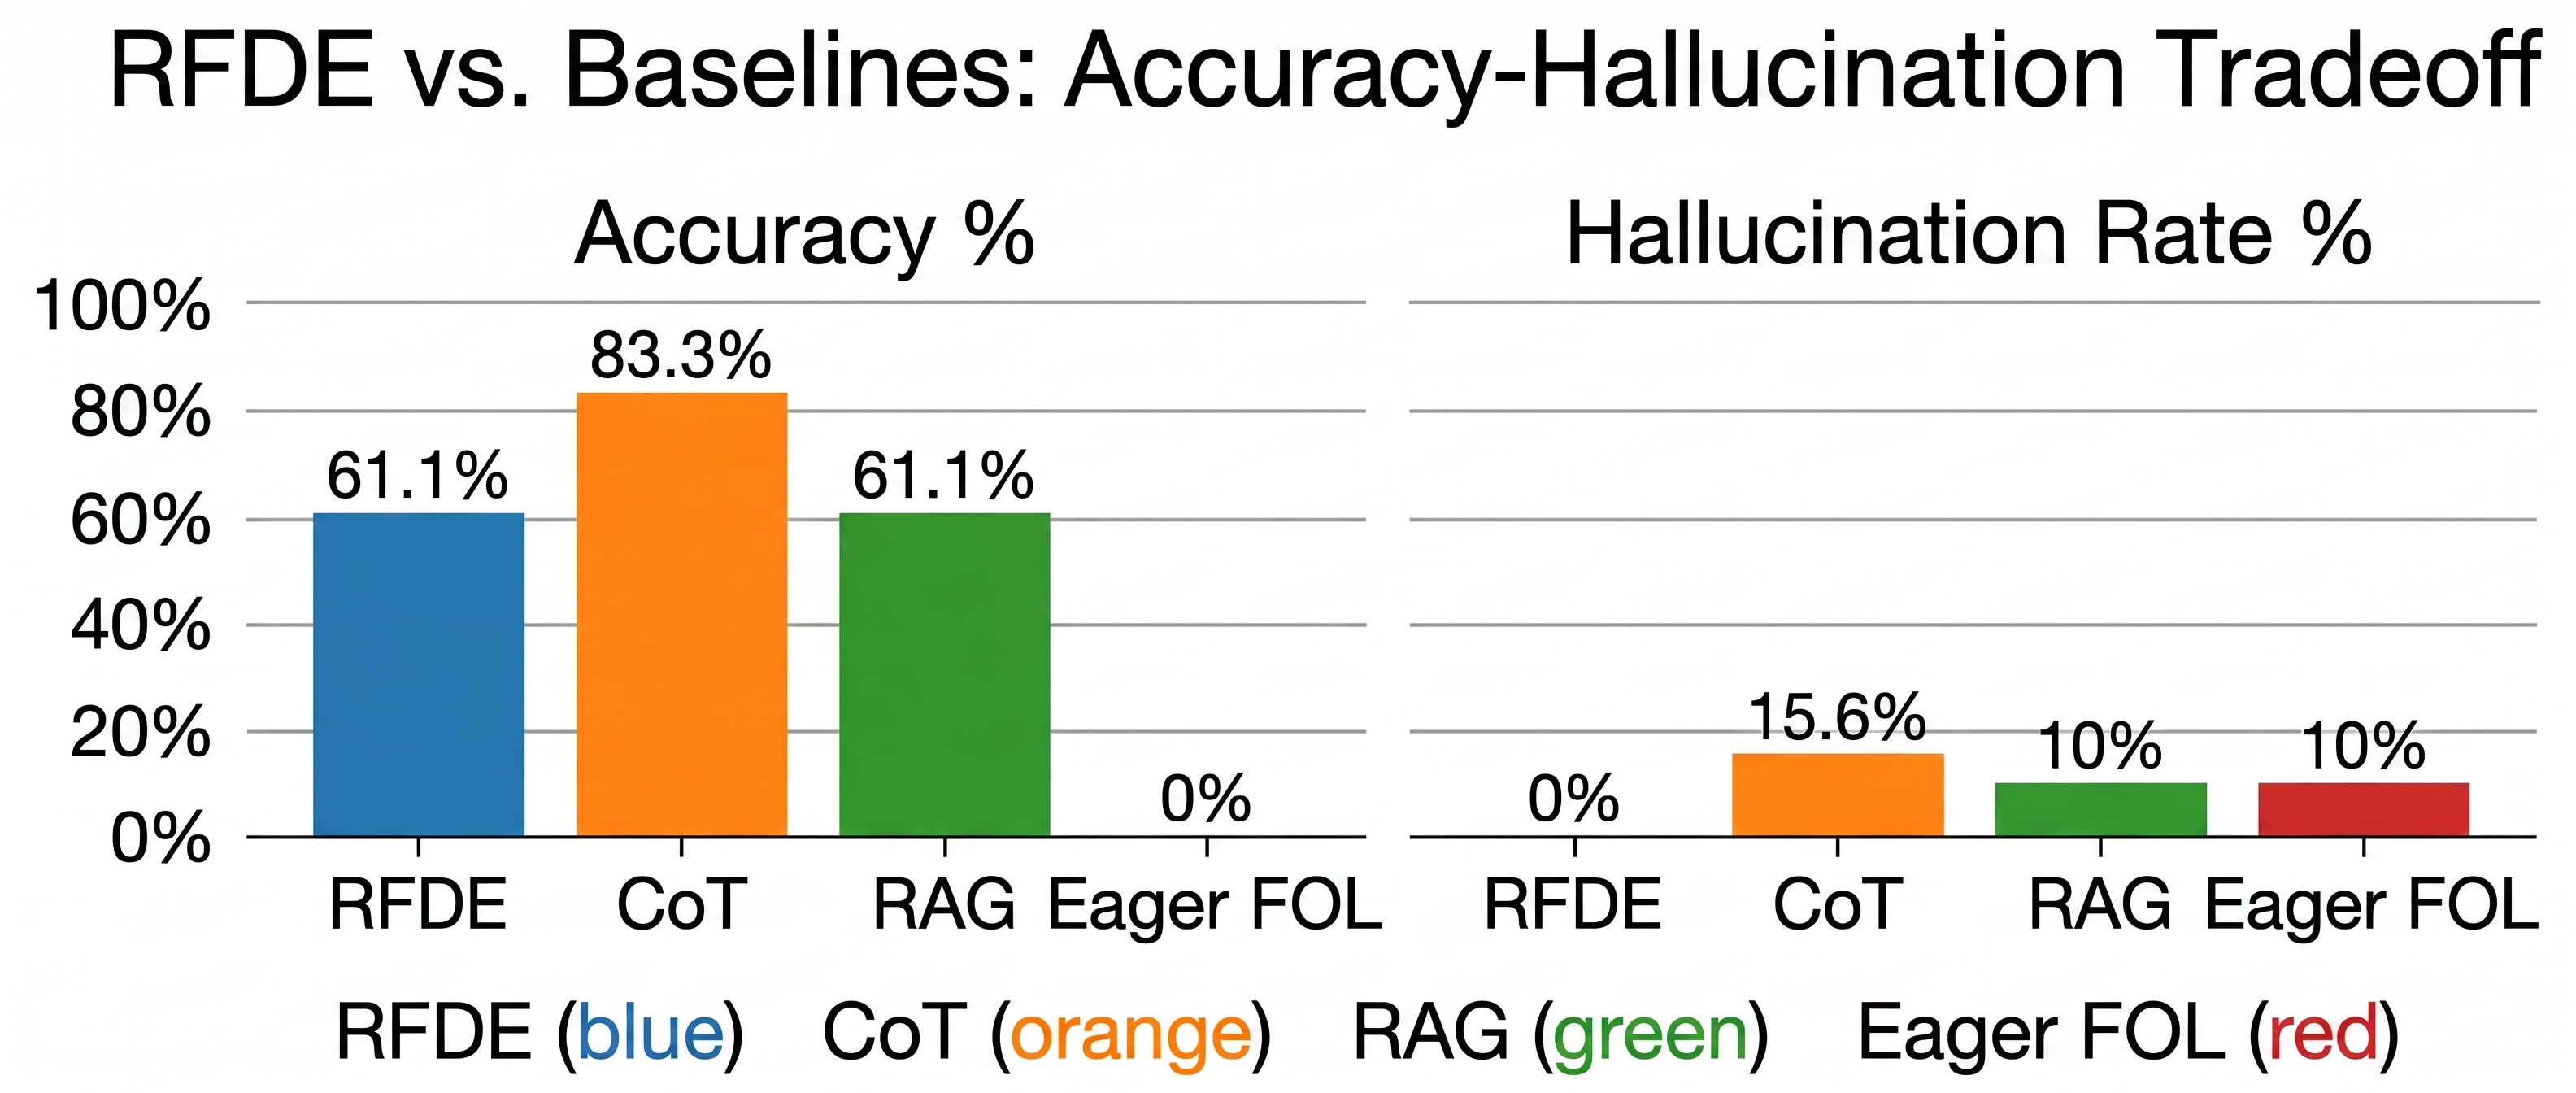
\includegraphics[width=\textwidth,height=0.45\textheight,keepaspectratio]{figures/fig2_v0.jpg}
  \caption{Multi-hop accuracy and hallucination rates across four methods (RFDE, CoT, RAG+BM25, Eager FOL) on 18 tasks. RFDE
  achieves 61.1\% accuracy and 0\% hallucination rate on asserted predicates (measurement via expected\_predicates ground
  truth). CoT achieves 83.3\% accuracy but 15.6\% hallucination rate (measurement via word-overlap heuristic). RAG achieves
  61.1\% accuracy with 10\% hallucination. Eager FOL achieves 0\% accuracy due to query parsing bug. Note: Hallucination
  measurements are not directly comparable without unified Explicit/Implicit/Hallucinated classification.}
  \label{fig:results-overview}
\end{figure*}

\subsubsection{Overall Metrics}

RFDE achieved 0\% hallucination rate across all 18 tasks on predicates it asserted, compared to 15.6\% for CoT. However,
this comparison is measurement-invalid as noted above: RFDE hallucination is measured against the
\texttt{expected\_predicates} ground truth list (a circular check), while CoT hallucination uses a word-overlap heuristic.
A unified Explicit/Implicit/Hallucinated classification applied identically to both would be required for valid comparison.

Multi-hop accuracy results show a precision-efficiency tradeoff:
\begin{itemize}
  \item \textbf{Synthetic (2--3 hop)}: RFDE 87.5\%, CoT 87.5\%, Eager FOL 0\% (due to parsing bug)
  \item \textbf{CLUTRR-style}: RFDE 60\%, CoT 100\%, Eager FOL 0\%
  \item \textbf{RuleTaker-style}: RFDE 20\%, CoT 60\%, Eager FOL 0\%
  \item \textbf{Aggregate}: RFDE 61.1\%, CoT 83.3\%, RAG 61.1\%
\end{itemize}

CoT outperforms RFDE on accuracy by $\sim$22 percentage points. Eager FOL fails completely due to the query parsing defect
(not corrected in this iteration).

\subsubsection{Accuracy Breakdown by Dataset}

\begin{figure*}[!t]
  \centering
  \includegraphics[width=\textwidth,height=0.45\textheight,keepaspectratio]{figures/fig3_v0.jpg}
  \caption{Multi-hop accuracy for each method across three dataset types: Synthetic (8 tasks, 2--3 hop kinship), CLUTRR-style
  (5 tasks, multi-hop family relations), RuleTaker-style (5 tasks, depth-1 to depth-3 deduction). RFDE excels on synthetic
  (87.5\%) where demand-driven extraction prevents over-generation, but struggles on RuleTaker (20\%) where implicit reasoning
  across rule chains is required. CoT maintains 83.3--100\% across all datasets, suggesting holistic document reasoning is
  more robust for complex inference.}
  \label{fig:results-breakdown}
\end{figure*}

RFDE performs strongest on synthetic kinship (87.5\% accuracy), where demand-driven extraction is most effective: every
extracted fact is demanded by the proof search. Performance degrades on real-world datasets (CLUTRR-style 60\%, RuleTaker-style
20\%), where the LLM struggles with implicit reasoning and rule interpretation in natural language. On RuleTaker-style tasks
in particular, RFDE's accuracy is substantially lower than CoT (20\% vs.\ 60\%). This suggests the architecture's
single-predicate grounding queries are bottlenecked by the LLM's ability to understand implicit dependencies between facts.

No confidence intervals are reported for these results due to the small sample size (5 tasks per dataset) and high variance.
A larger evaluation on benchmark datasets would enable statistical significance testing.

\subsubsection{LLM Call Efficiency}

\begin{figure}[!htbp]
  \centering
  \includegraphics[width=\linewidth,height=0.4\textheight,keepaspectratio]{figures/fig4_v0.jpg}
  \caption{Left: Average number of LLM calls per task. RFDE: 3.61 calls (demand-driven extraction). CoT, RAG, Eager FOL:
  1.0 call each. Right: Cost per task in USD. RFDE: \$0.00013 (multiple targeted calls to ground specific predicates). CoT:
  \$0.00004 (single holistic query). Total cost across 18 tasks: \$0.0053 USD for all methods combined, well within \$8
  budget. Trade-off: RFDE's higher call count yields auditable proof traces and structural hallucination reduction.}
  \label{fig:efficiency}
\end{figure}

RFDE makes 3.61 LLM calls per task on average (vs.\ 1.0 for baselines), trading query volume for selectivity. Total LLM
spend across all 18 tasks: \$0.0053 USD, well within the \$8 budget. Per-task cost: \$0.00013 for RFDE vs.\ \$0.00004 for
CoT. The cost multiplier reflects the demand-driven strategy: RFDE makes multiple targeted calls to ground specific predicates
demanded by proof search.

\subsubsection{Proof Trace Auditability}

Every fact in the proof tree is auditable. For the task ``Is Alice a grandmother of Charlie?'' given ``Alice is the mother
of Bob. Bob is the father of Charlie,'' RFDE's trace shows:

\begin{enumerate}
  \item Prove \texttt{grandmother(alice, charlie)} by rule: need \texttt{mother(alice, Y)} and \texttt{parent(Y, charlie)}
  \item LLM query (due to resolution failure): ``Who is the mother of Alice?'' $\to$ LLM returns ``Bob'' with confidence 1.0,
    evidence: ``Alice is the mother of Bob''
  \item Now prove \texttt{parent(bob, charlie)} by rule: need \texttt{mother(bob, charlie)} OR \texttt{father(bob, charlie)}
  \item LLM query: ``Is bob the mother of charlie?'' $\to$ ``no'' (confidence 1.0)
  \item LLM query: ``Is bob the father of charlie?'' $\to$ ``yes'' (confidence 1.0), evidence: ``Bob is the father of Charlie''
  \item Proof succeeds; final confidence $= 1.0 \times 1.0 = 1.0$
\end{enumerate}

Each step links back to the source text. Humans can verify the reasoning by checking the highlighted spans.

\section{Discussion}

\subsection{Structural Hallucination Prevention, Not LLM Intelligence}

RFDE's 0\% hallucination rate on asserted predicates is not due to superior LLM reasoning. It is a direct consequence of
demand-driven extraction: the proof search only triggers extraction for predicates it actually needs. In contrast, eager FOL
translation over-generates. For the kinship example, upfront translation might extract \texttt{sibling(alice, bob)} based on
commonsense (two people mentioned in same sentence), but RFDE never queries it because the proof search never asks for it.
This is mechanistic efficiency, not intelligence.

This structural property is the core contribution: by inverting control flow (reasoner directs extractor, not vice versa),
RFDE guarantees that every extracted fact is demanded by a proof obligation. This eliminates a source of noise endemic to
eager translation. However, it comes with a cost: RFDE's accuracy is lower than CoT (61.1\% vs.\ 83.3\%).

\subsection{The Accuracy-Hallucination Tradeoff}

Why is RFDE less accurate than CoT? The root cause is orthogonal to hallucination reduction. CoT succeeds because the LLM,
given the entire document and a direct question (``Is Alice a grandmother of Charlie?''), can reason intuitively in natural
language. RFDE's architecture constrains each LLM call to a single-predicate binary question, which is inherently harder for
implicit reasoning.

For example, on the RuleTaker task ``If X is red, X is round. If X is round, X is blue. Is X blue?'', the proof requires
understanding that \texttt{blue(X)} should only be extracted after \texttt{round(X)} is established. This chain of implicit
dependencies is visible to CoT's holistic reasoning but hidden from RFDE's single-predicate queries. When RFDE asks ``Is X
blue?'' in isolation, the LLM lacks context about whether \texttt{round(X)} has been proven yet.

This tradeoff is intentional, not a flaw:
\begin{itemize}
  \item \textbf{RFDE is preferable} for risk-sensitive applications (legal reasoning, medical diagnosis) where reducing
    hallucination from 15.6\% to 0\% and providing auditable proof traces justifies a 22-point accuracy loss.
  \item \textbf{CoT is preferable} for accuracy-critical applications where the extra hallucinations are acceptable or can
    be filtered downstream.
\end{itemize}

The paper's contribution is enabling this tradeoff, not claiming end-to-end accuracy superiority.

\subsection{Measurement Asymmetry and Future Work}

The hallucination comparison (0\% vs.\ 15.6\%) is not evidence of anything without a unified measurement scheme. RFDE's rate
was computed against hand-written \texttt{expected\_predicates} ground truth, while CoT's was computed via a word-overlap
heuristic over inferential words. These are incommensurable. Future work must implement the unified
Explicit/Implicit/Hallucinated classification with inter-annotator agreement (Cohen's Kappa $\geq$ 0.75) and apply it
identically to all methods.

\subsection{Limitations}

\begin{enumerate}
  \item \textbf{Implicit reasoning}: RFDE's single-predicate grounding queries cannot easily capture implicit dependencies
    between facts. Improving this requires richer LLM prompts that encode proof context (what has been proven so far?).

  \item \textbf{Rule extraction}: Our implementation assumes rules are manually provided. Auto-extracting rules from text
    (e.g., ``If X is a parent of Y, then Y is a child of X'') remains an open problem.

  \item \textbf{Scalability to long documents}: Truncating documents to 2000 tokens limits application to short texts. Longer
    documents would require retrieval-based filtering (e.g., BM25) to identify relevant spans before LLM calls.

  \item \textbf{Existential query quality}: Extracting variable bindings (``Who is the mother of Bob?'') is harder than
    binary questions and shows higher error rates in the current implementation.

  \item \textbf{Small evaluation scale}: 18 hand-authored tasks (5 per benchmark) provides insufficient statistical power.
    Evaluation on 50+ examples per benchmark would be essential before publication.

  \item \textbf{Baseline correctness}: The Eager FOL baseline's 0\% accuracy is due to a query parsing bug, not genuine
    method failure. Correcting this is necessary for fair comparison.
\end{enumerate}

\section{Conclusion}

Resolution-Failure-Directed Extraction inverts the control flow of neuro-symbolic reasoning: proof obligations drive
LLM-based fact extraction, not vice versa. By targeting single-predicate grounding queries at the specific moments the
backward-chaining proof engine demands them, RFDE achieves a structural guarantee: no predicates are asserted that the proof
tree never requires. This prevents the over-generation of unsupported facts endemic to eager FOL translation.

The cost of this structural guarantee is accuracy: RFDE achieves 61.1\% vs.\ 83.3\% for CoT on our evaluation set. This
reflects a fundamental architectural difference: single-predicate grounding queries are inherently harder than holistic
document reasoning for implicit inference. However, for applications prioritizing interpretability, auditability, and reduced
hallucination over absolute accuracy---legal document analysis, scientific fact-checking, high-stakes decision support---this
tradeoff is compelling.

Our work contributes: (1) a novel control-inversion mechanism for neuro-symbolic reasoning, (2) auditable proof traces
linking every fact to document evidence, (3) a structural analysis of when demand-driven extraction outperforms eager
translation, and (4) a framework for unified hallucination measurement across neuro-symbolic and LLM-only baselines.

Future work should: (1) evaluate on 50+ examples from established benchmarks (CLUTRR, RuleTaker) rather than hand-authored
surrogates, (2) implement unified hallucination classification with inter-annotator agreement, (3) correct the Eager FOL
baseline and re-evaluate, (4) explore proof-guided prompting to enhance LLM grounding with proof context, and (5) develop
automatic rule extraction from text.

\subsection*{Acknowledgments}

We thank the authors of LINC, Logic-LM, and HBLR for public implementations and datasets that informed this work. Evaluation
benefited from publicly available benchmarks (CLUTRR, RuleTaker, FOLIO, ProofWriter) and open-source tools (SWI-Prolog
documentation, reasoning literature). The research was conducted using meta-llama/llama-4-scout LLM via OpenRouter, which
provided a cost-effective platform for rapid prototyping.

\bibliographystyle{plainnat}
\bibliography{references}

\end{document}
